\documentclass[10pt,a4paper]{article}
\usepackage{rpgcover}
\usepackage{illustrated-panel}
\usepackage{longtable,booktabs}
\usepackage{float}
\usepackage{multicol}
\usepackage{fancyvrb}
\usepackage{wrapfig}
\usepackage{needspace}
\usepackage{titlesec}
\babelprovide[import]{italian}
\titleformat{\subsection}{\normalfont\Large\bfseries\color{rpgbrown}}{}{0pt}{}
\titlespacing*{\subsection}{0pt}{12pt plus 2pt}{5pt}
\titleformat{\subsubsection}{\normalfont\normalsize\bfseries\color{rpgbrown}}{}{0pt}{}
\titlespacing*{\subsubsection}{0pt}{10pt plus 2pt}{4pt}
\usepackage{etoolbox}
\usepackage{xsavebox}
% Stat boxes never start in the last lines of a page, where they would split after their title.
\BeforeBeginEnvironment{rpgnote}{\par\needspace{8\baselineskip}}
\pretocmd{\subsection}{\needspace{5\baselineskip}}{}{}
\pretocmd{\subsubsection}{\needspace{4\baselineskip}}{}{}
\setcounter{tocdepth}{1}
\clubpenalty=10000
\widowpenalty=10000
\displaywidowpenalty=10000
\interlinepenalty=0
\emergencystretch=1.2em
\newcommand{\HHInlineFigure}[3]{%
  \begin{center}\includegraphics[width=#2\linewidth,height=56mm,keepaspectratio]{assets/hollow-hearth/#1.jpg}%
  \par\vspace{2pt}{\footnotesize\itshape\color{rpgbrown}#3\par}\end{center}}
% Scene-opening illustrations float: here when they fit, otherwise at the foot of the next page.
% They never narrow a read-aloud box or leave a gap at the bottom of a page.
\newcommand{\HHSceneArt}[2]{%
  \begin{figure}[!hb]\centering\includegraphics[width=.62\linewidth,height=58mm,keepaspectratio]{assets/hollow-hearth/#1.jpg}%
  \par\vspace{2pt}{\footnotesize\itshape\color{rpgbrown}#2\par}\end{figure}}
% Full-page maps float to the next free page instead of ending the current page early.
\newcommand{\HHSceneMap}[3]{%
  \begin{figure}[p]\centering
    {\Large\bfseries\color{rpgbrown}#2\par}\vspace{6mm}%
    \includegraphics[width=.96\linewidth,height=190mm,keepaspectratio]{assets/hollow-hearth/#1.jpg}\par\vspace{4mm}%
    {\small\itshape\color{rpgbrown}#3\par}%
  \end{figure}}
\newcommand{\HHContents}{%
  \clearpage\thispagestyle{rpg}
  \vspace*{10mm}\begin{center}{\fontsize{27}{31}\selectfont\bfseries INDICE\par}\vspace{9pt}
  {\color{rpgline}\rule{.76\linewidth}{.55pt}}\end{center}\vspace{9mm}
  \begingroup
  \expandafter\def\csname l@section\endcsname##1##2{\csname @dottedtocline\endcsname{1}{0em}{4em}{\bfseries ##1}{##2}}%
  \csname @starttoc\endcsname{toc}\endgroup
  \vspace{5mm}
  \begin{center}\resizebox{!}{68mm}{\xusebox{HHFrontOverlay}}\end{center}
  \vfill
  \begin{center}{\small\itshape Un'avventura di Jacopo Biscella\par}\vspace{5pt}
  {\footnotesize Questa avventura è pubblicata con licenza Creative Commons Attribuzione-Condividi allo stesso modo 4.0 Internazionale (CC BY-SA 4.0), alle stesse condizioni di All'ultimo tiro. È consentita la condivisione e l'adattamento, anche commerciale, purché l'autore venga citato e le opere derivate mantengano la stessa licenza.\par}\end{center}
  \clearpage}
\RPGSetRunningTitle{La campana di Focolare Vuoto}
\RPGSetCoverWordSpace{.78em}
% JPEG copies of the shared cover backgrounds (scripts/build-adventure-print-art.sh): the PNGs
% made each PDF about 6 MB larger with no visible difference in print.
\RPGSetFrontBackground{assets/engraved-front-background.jpg}\RPGSetBackBackground{assets/engraved-cover-background.jpg}
\hypersetup{pdftitle={La campana di Focolare Vuoto},pdfauthor={Jacopo Biscella}}
\setlength{\emergencystretch}{2em}
\setcounter{secnumdepth}{-1}
\newcommand{\tightlist}{\setlength{\itemsep}{0pt}\setlength{\parskip}{0pt}}

\newcommand{\HHFrontArt}{assets/hollow-hearth/front-overlay.png}
\newcommand{\HHBackArt}{assets/hollow-hearth/back-overlay.png}
% Existing rpgcover.sty is used unchanged; only an adventure-specific back-cover layout follows.

\setlength{\parskip}{3pt plus .5pt minus .5pt}
\linespread{1.06}\selectfont
\newcommand{\HHAdventureBackCover}{%
 \clearpage\pagenumbering{gobble}\RPGCoverPagetrue\thispagestyle{empty}\null
 \begin{tikzpicture}[remember picture,overlay,x=1mm,y=1mm]
  \RPGDrawBackground{\RPGBackBackgroundFile}
  \node[align=center,text=coverink,text width=170mm,inner sep=0pt] at ($(current page.south west)+(105mm,260mm)$)
    {{\RPGCoverTitleFont\fontsize{19}{23}\selectfont\spaceskip=\RPGCoverWordSpace\relax LA CAMPANA DI FOCOLARE VUOTO}};
  \draw[coverink,line width=.45pt] ($(current page.south west)+(57mm,246mm)$)--($(current page.south west)+(153mm,246mm)$);
  \node[anchor=north,align=left,text=coverink,text width=137mm,inner sep=0pt] at ($(current page.south west)+(105mm,240mm)$)
    {\RPGCoverTextFont\fontsize{10.4}{13.4}\selectfont
    Sette generazioni fa, un Mistico errante benedisse una campana di bronzo. Il villaggio dove finisce la strada del Re e inizia la foresta prese il nome di Focolare Vuoto. Al crepuscolo, la campana teneva lontano il Popolo Cavo, creature pallide dalla pelle di corteccia che sussurrano tra gli alberi.};
  \node[anchor=north,align=center,text=coverink,text width=140mm,inner sep=0pt] at ($(current page.south west)+(105mm,197mm)$)
    {\RPGCoverSubtitleFont\fontsize{13}{17}\selectfont Tre notti fa, la campana è stata rubata.\\[4pt]
    La prossima notte senza luna sarà fra quarantotto ore.};
  \draw[coverink,line width=.45pt] ($(current page.south west)+(57mm,167mm)$)--($(current page.south west)+(153mm,167mm)$);
  \node[anchor=north,align=left,text=coverink,text width=137mm,inner sep=0pt] at ($(current page.south west)+(105mm,162mm)$)
    {\RPGCoverTextFont\fontsize{9.9}{12.1}\selectfont
    Un'avventura introduttiva per All'ultimo tiro, per tre o quattro Protagonisti, da giocare in due o tre ore. Insegna i gradini dei tiri, le distanze narrative, le Ferite, la Stanchezza, la magia e il Contraccolpo.};
  \node[anchor=north,align=center,text=coverink,text width=147mm,inner sep=0pt] at ($(current page.south west)+(105mm,133mm)$)
    {\RPGCoverSubtitleFont\fontsize{10.5}{13.2}\selectfont
     Tre approcci. Un finale scelto dal gruppo.\\
     Un cavaliere caduto in disgrazia. Un compratore misterioso.\\
     Una decisione da prendere insieme.};
  \node[anchor=north,align=center,text=coverink,text width=144mm,inner sep=0pt] at ($(current page.south west)+(105mm,114mm)$)
    {\RPGCoverTextFont\fontsize{10.2}{12.5}\selectfont
     Contiene: quattro mappe $\cdot$ cinque illustrazioni $\cdot$\\ un promemoria per il Narratore.};
  \RPGOptionalArtwork{105}{59}{130}{24}{\HHBackArt}
  \filldraw[fill=white,draw=coverink,line width=.55pt]
    ($(current page.south west)+(139mm,25mm)$) rectangle
    ($(current page.south west)+(187mm,55mm)$);
 \end{tikzpicture}
 \clearpage\RPGCoverPagefalse
}
\newcommand{\HHFrontCover}{%
 \clearpage\RPGCoverPagetrue\thispagestyle{empty}\null
 % The front overlay goes into the PDF once, as a form reused on the contents page.
 \xsavebox{HHFrontOverlay}{\includegraphics{\HHFrontArt}}
 \begin{tikzpicture}[remember picture,overlay,x=1mm,y=1mm]
  \RPGDrawBackground{\RPGFrontBackgroundFile}
  \node[align=center,text=coverink,text width=138mm,inner sep=0pt]
   at ($(current page.south west)+(105mm,248mm)$)
   {\RPGCoverTitleFont\fontsize{16.6}{20.7}\selectfont\spaceskip=\RPGCoverWordSpace\relax LA CAMPANA DI\\[1.0mm]FOCOLARE VUOTO};
  \node[align=center,text=coverink,text width=135mm,inner sep=0pt]
   at ($(current page.south west)+(105mm,235mm)$)
   {\RPGCoverSubtitleFont\fontsize{9.5}{12}\selectfont Un'avventura per «All'ultimo tiro»};
  \node[inner sep=0pt,anchor=center] at ($(current page.south west)+(105mm,119mm)$)
   {\resizebox{!}{138mm}{\xusebox{HHFrontOverlay}}};
  \node[align=center,text=coverink,text width=124mm,inner sep=0pt]
   at ($(current page.south west)+(105mm,25mm)$)
   {\RPGCoverTextFont\fontsize{12}{15}\selectfont Jacopo Biscella};
 \end{tikzpicture}\clearpage\RPGCoverPagefalse}
\begin{document}
% Select the language here: babel resets to its main language (english) at \begin{document}.
\selectlanguage{italian}
\RPGStartFrontMatter
\HHFrontCover
\HHContents
\RPGStartMainMatter
\RPGChapter{La campana di Focolare Vuoto}
\begin{center}\textit{Un'avventura introduttiva per All'ultimo tiro}\par\smallskip
\small 2--3 ore \textperiodcentered\ 3--4 Protagonisti \textperiodcentered\ Almeno un Combattente \textperiodcentered\ Edizione del Narratore
\end{center}
\noindent\textit{I quattro Protagonisti pregenerati sono pubblicati con i download di questa avventura: un PDF per ogni scheda, basata sul modello di scheda del manuale.}\par\medskip
\subsection{Una parola al Narratore}\label{una-parola-al-narratore}

Questa avventura è anzitutto uno strumento didattico e poi una storia. Ogni scena mette in primo piano un elemento portante di \emph{All'ultimo tiro}, senza mai interrompere la finzione per fare lezione. Quando scorreranno i titoli di coda, i tuoi giocatori avranno sperimentato i gradini dei tiri, le distanze narrative, il pool unico di Ferite e Stanchezza, l'Aiuto e --- se avrai fatto bene il tuo lavoro --- almeno uno Sforzo dichiarato con mano tremante, proprio nel momento promesso dal titolo.

Il ritmo indicativo è all'incirca questo:

\begin{itemize}
\tightlist
\item
  30 minuti per la creazione dei personaggi e i preparativi \emph{(usa le regole di creazione del manuale, pp. 2--6)}
\item
  35 minuti per \textbf{Scena 1 · Il villaggio} (indagine sociale)
\item
  40 minuti per \textbf{Scena 2 · Il bosco dei sussurri} (prova di abilità + atmosfera)
\item
  60 minuti per \textbf{Scena 3 · La vecchia torre} (combattimento culminante + risoluzione)
\item
  10 minuti per \textbf{Le tre domande} e le conseguenze
\end{itemize}

Un promemoria che vale la pena ripetere: in questo gioco non ci sono tiri di iniziativa, né un ordine di turno fisso, né una griglia. Le mappe incluse nell'avventura sono ancore spaziali per l'immaginazione di tutti: al tavolo le distanze sono sempre \textbf{Addosso}, \textbf{Vicino}, \textbf{A portata} o \textbf{Lontano}.

\par\vspace{3pt}

\subsection{Che cosa insegna l'avventura}\label{che-cosa-insegna-lavventura}

\begingroup\setlength{\arrayrulewidth}{.34pt}\arrayrulecolor{rpgline}\renewcommand{\arraystretch}{1.32}\rowcolors{2}{rpgshade}{white}\par\smallskip\noindent\begin{tabularx}{\linewidth}{|Y|Y}\hline
\rpghead{Scena} & \rpghead{Meccaniche introdotte} \\ \hline
Il villaggio & Tiri di Caratteristica + Abilità; VR per le azioni sociali; tiri contrapposti; uso di Tratto e Fardello \\ \hline
Il bosco dei sussurri & Aiuto; Condizioni ($-1$ gradino); fasce di distanza narrative \\ \hline
La vecchia torre & Combattimento; Ferite e Stanchezza; Critico; Contraccolpo; \textbf{Sforzo}; conseguenze \\ \hline
\end{tabularx}\arrayrulecolor{black}\endgroup\par\smallskip

Se il gruppo comprende un Mistico, è probabile che nella Scena 3 avvenga anche il suo primo Contraccolpo: lascia che accada.

\par\vspace{3pt}

\par\needspace{65mm}\subsection{La premessa}\label{la-premessa}

\begin{wrapfigure}{r}{.38\linewidth}\vspace{-5pt}\centering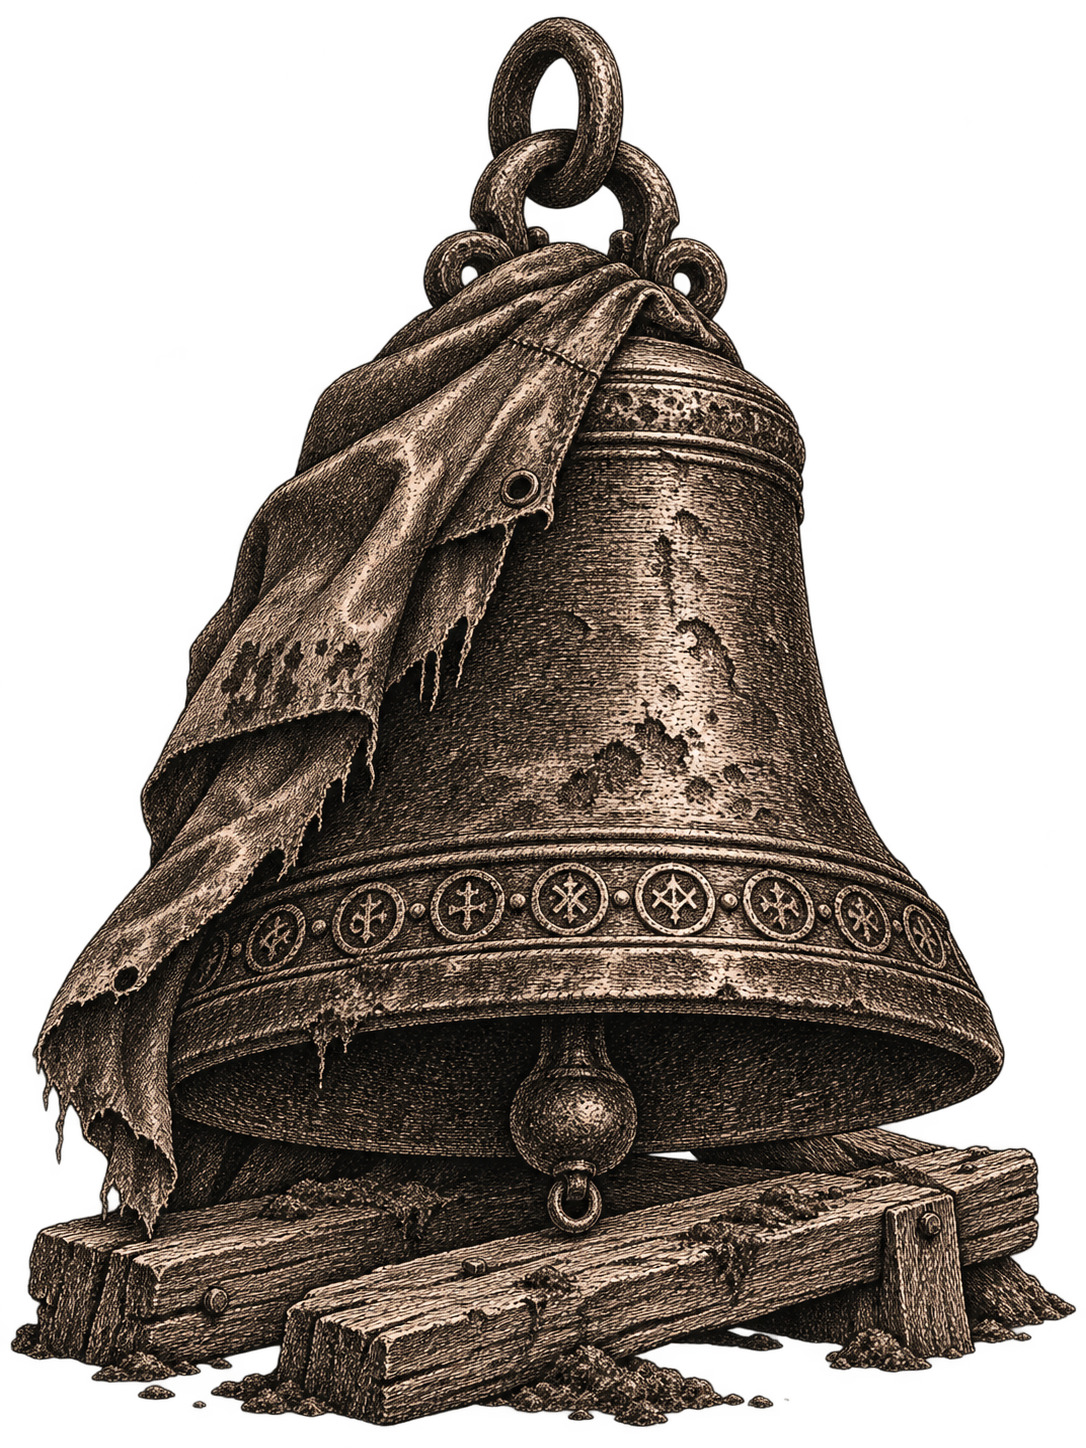
\includegraphics[width=.98\linewidth,height=58mm,keepaspectratio]{assets/hollow-hearth/bell.jpg}\par{\scriptsize\itshape\color{rpgbrown}La campana rubata, avvolta nella tela cerata}\vspace{-5pt}\end{wrapfigure}

Sette generazioni fa, un Mistico errante di nome \textbf{Veyl Ashen} benedisse una campana di bronzo fusa nella forgia di un piccolo insediamento, sorto dove finisce la strada del Re e comincia l'antica foresta. L'insediamento prese il nome di \textbf{Focolare Vuoto}. La campana, suonata a ogni crepuscolo, teneva il \textbf{Popolo Cavo} --- esseri pallidi dalla pelle di corteccia che sussurrano fra gli alberi --- confinato fra le radici, dove deve stare.

Tre notti fa, la campana è stata rubata.

Una banda di briganti guidata da un disertore che si fa chiamare \emph{«Ser»} \textbf{Corwin Vask} è scesa dalle rovine della torre di guardia dove si accampa, ha ucciso l'apprendista del vecchio campanaro ed è scomparsa nel bosco verso nord, con la campana avvolta in una tela cerata. Gli abitanti hanno seppellito il ragazzo ieri mattina.

La prossima notte senza luna arriverà fra \textbf{quarantotto ore}.

Questo è il conto alla rovescia. Quella notte, dopo il tramonto della luna, senza una campana da suonare al crepuscolo, il Popolo Cavo tornerà in un Focolare Vuoto che ha dimenticato come difendersi.

\par\vspace{3pt}

\subsection{L'aggancio}\label{laggancio}

\HHSceneArt{village}{Focolare Vuoto al crepuscolo: la piattaforma vuota}

Adatta l'arrivo ai Tratti e ai Fardelli scritti dai giocatori. Qualche spunto rapido:

\begin{itemize}
\tightlist
\item
  Un \textbf{Erudito} che segue la discendenza di Veyl Ashen negli antichi registri liturgici.
\item
  Un \textbf{Avventuriero} che porta un contratto dal paese successivo lungo la strada.
\item
  Un \textbf{Mistico} che ha \emph{sentito} la campana ammutolire a leghe di distanza.
\item
  Un \textbf{Combattente} che si allontana da un campo di battaglia sul quale non vuole più stare.
\end{itemize}

Qualunque sia la strada che li porta qui, la sindaca del villaggio, \textbf{Hesta Thrush}, offrirà loro quel poco che Focolare Vuoto possiede --- monete, ospitalità e una reliquia conservata fin dalla fondazione (vedi \emph{Risoluzione}) --- per riportare a casa la campana.

\begin{quote}
\subsubsection{Da leggere ad alta voce --- L'arrivo}\label{da-leggere-larrivo}

\emph{La strada si restringe in una pista, la pista in un sentiero, e il sentiero sbuca in una radura di basse case di pietra dai ripidi tetti d'ardesia. Al centro della piazza sorge una piattaforma di legno. Vuota. Quattro bulloni di ferro, là dove qualcosa di pesante è stato strappato via. Dai camini non esce fumo. In piazza non c'è nessuno.}

\emph{Poi una porta si apre, ne esce un'anziana donna e, alle sue spalle, sentite qualcuno piangere.}
\end{quote}

\par\vspace{3pt}

\HHSceneMap{map-village}{Focolare Vuoto: pianta del villaggio}{La piattaforma della campana è nella piazza; Hesta, Bram, Vela e la locanda sono lì vicino. Tutti i luoghi del villaggio: Vicino.}
\RPGChapter{Scena 1 --- Il villaggio}\label{scena-1-il-villaggio}

\textbf{Focus meccanico:} tiri di Sapienza, bonus delle Abilità, tiri contrapposti, uso di Tratto e Fardello.

A Focolare Vuoto ci sono tre persone che contano per l'indagine. I Protagonisti possono parlare con tutte e tre, nell'ordine che preferiscono. Ognuna possiede un pezzo del quadro, e almeno una di loro sta \emph{quasi} mentendo.

\par\smallskip\begin{rpgnote}[fontupper=\normalfont]\textbf{PNG del villaggio}\par\smallskip
\textbf{Hesta Thrush} \emph{(PNG)} --- Sapienza Competente. Nessuna statistica di combattimento: se la violenza la raggiunge, è esattamente ciò che sembra.\par\smallskip
\textbf{Vela Roan} \emph{(PNG)} --- Sapienza Esperto (Erboristeria, Sopravvivenza), Prodigio Competente. Non combatte se non è messa alle strette.\par\smallskip
\textbf{Il vecchio Bram} \emph{(PNG)} --- Sapienza Competente. Non è più in grado di combattere.\end{rpgnote}\par\smallskip
Usa \textbf{la mappa del villaggio di Focolare Vuoto} per la disposizione. Tutti i luoghi del villaggio sono a distanza \textbf{Vicino} l'uno dall'altro.

\subsubsection{Hesta Thrush --- La sindaca}\label{hesta-thrush-la-sindaca}

Una donna sulla sessantina, segnata dalle intemperie, consumata dal dolore. Suo figlio partì per la guerra e non tornò mai; è sindaca da undici anni e conosce ogni abitante del villaggio fino al secondo nome.

Ciò che racconta liberamente:

\begin{itemize}
\tightlist
\item
  I briganti sono venuti dalla \textbf{vecchia torre}, a quattro ore di cammino verso nord, dentro il bosco dei sussurri.
\item
  Come ricompensa finale del villaggio offre una reliquia della fondazione: la \textbf{Lama del Sale} \emph{(manuale, p. 8)}.
\end{itemize}

Ciò su cui mentirà:

Sa che suo cugino \textbf{Marrel} è stato visto bere con uno dei briganti alla locanda, la settimana prima del furto. Non vuole che il cugino finisca impiccato per questo. Un \textbf{tiro di Sapienza contrapposto alla Sapienza (Competente) di Hesta} coglie il suo disagio. \textbf{Diplomazia} la convince a confessare; lo stesso vale per \textbf{Retorica}. Funziona anche \textbf{Intimidire, VR 5}, ma per il resto dell'avventura il villaggio si schiererà contro il gruppo.

\begin{quote}
\subsubsection{Spunto per Tratto/Fardello}\label{spunto-per-tratto-e-fardello}

Un Protagonista il cui Fardello riguarda la guerra, figli perduti o giuramenti infranti troverà in Hesta un'alleata oppure uno specchio. Sfruttalo. \emph{«Mi ricordi lui»}, dice, guardando la persona sbagliata.
\end{quote}

\subsubsection{Il vecchio Bram --- Il campanaro}\label{il-vecchio-bram-il-campanaro}

Il campanaro, sulla ottantina, è sopravvissuto perché all'arrivo dei briganti si era appartato fra i rovi per un bisogno. Il ragazzo ucciso era il suo apprendista e il suo pronipote. È furioso. Non a voce alta. L'altro tipo di furia.

Ciò che ha visto:

\begin{itemize}
\tightlist
\item
  Quattro uomini. Uno in armatura, uno con un arco lungo, due con pugnali.
\item
  Quello in armatura aveva \textbf{un sole bianco cucito sulla spalla del mantello}: lo stemma di un ordine cavalleresco caduto in disgrazia dieci anni fa. Un \textbf{tiro di Sapienza, VR 4 con l'Abilità Storia}, identifica l'ordine come l'\textbf{Ordine del Sole Pallido}, sciolto per «trasgressioni rituali» durante le guerre. Senza Storia serve \textbf{VR 5} per ripescare un vago ricordo.
\item
  Crede che la campana sia viva. Potrebbe avere ragione.
\end{itemize}

\subsubsection{Vela Roan --- L'erborista}\label{vela-roan-lerborista}

Quarant'anni, sveglia e tagliente, è l'unica persona del villaggio che sia entrata \emph{dentro} il bosco dei sussurri e ne sia tornata. Sa che cosa sia il Popolo Cavo. Non lo dirà apertamente. Parla per storie.

Ciò che offre, a chi sa chiederlo nel modo giusto:

\begin{itemize}
\tightlist
\item
  Il «popolo di corteccia» sale dalle radici quando nessuna campana suona. Crede che uno del Popolo Cavo cammini già fra gli abitanti sotto sembianze umane.
\item
  Darà una fiala di \textbf{radicenotte distillata} --- \emph{un oggetto notevole: versata su una lama, il colpo successivo infligge +1 Ferita contro le creature innaturali; un solo uso} --- \textbf{se} un Protagonista accetta di portarle un rametto di \textbf{fiore d'argento lunare} dal cuore del bosco.
\end{itemize}

Quest'ultima è una tentazione secondaria: un'occasione per un momento di Fardello se qualcuno in seguito manca alla parola data, o per mettere alla prova un Tratto d'onore. Il fiore esiste. Sta al gruppo decidere se trovare il tempo per cercarlo.

\subsubsection{Opzionale · Marrel, il cugino}\label{opzionale-marrel-il-cugino}

Se i Protagonisti seguono la bugia di Hesta, trovano Marrel alla locanda, intento ad annegare la paura nel bere. Conferma che il brigante con cui aveva parlato --- un uomo di nome \textbf{Thessik} --- si vantava di un compratore che \emph{«paga in argento del nord»} e che sarebbe venuto per la campana. Marrel non sapeva che sarebbe stata rubata. \textbf{Intimidire, VR 4}, lo fa crollare. Funziona anche \textbf{Diplomazia, VR 4}, offrendogli da bere. \textbf{Commercio, VR 4}, se un Erudito vuole ragionare su che cosa significhi davvero «argento del nord» (è un'espressione dei contrabbandieri che attraversano il confine: l'argento del nord non esiste, è un nome in codice per l'oro fatato).

\subsubsection{Nota didattica per il Narratore}\label{nota-didattica-per-il-narratore}

Quando un giocatore dichiara \emph{«Voglio capire se mente»}, chiedigli \textbf{come}. La incalza? La osserva? La coglie in contraddizione? Il \emph{come} determina Caratteristica e Abilità. \textbf{Sapienza} è la scelta predefinita per leggere una persona; \textbf{Etichetta} la coglie in uno scivolone cortese, \textbf{Intimidire} la spinge a sbagliare, \textbf{Inganno} ti permette di mentire meglio di lei fino a metterla all'angolo. Non esiste un sottosistema separato di combattimento sociale. C'è soltanto Sapienza più un'Abilità pertinente contro un VR. Come per tutto il resto.

\par\vspace{3pt}

\HHSceneMap{map-forest}{Attraverso il bosco dei sussurri}{Il villaggio in basso, la torre in alto; il Popolo Cavo appare sulla sponda che il gruppo ha appena lasciato.}

\RPGChapter{Scena 2 --- Il bosco dei sussurri}\label{scena-2-il-bosco-dei-sussurri}

\HHSceneArt{hollow}{Un osservatore fra gli alberi}

\textbf{Focus meccanico:} Aiuto, fasce di distanza, Condizioni come $-1$ gradino.

Un sentiero di felci schiacciate e brandelli di tela cerata caduti conduce a nord dal villaggio. Il bosco dei sussurri lo inghiotte nel giro di cinquanta passi. Qui gli alberi si piegano verso l'interno.

\begin{quote}
\subsubsection{Da leggere ad alta voce --- Entrare nel bosco}\label{da-leggere-entrare-nel-bosco}

\emph{Appena superate il limitare degli alberi, la luce cala di un terzo. Non per colpa delle fronde --- non ci sono fronde degne di questo nome --- ma come se l'aria stessa la bevesse. I suoni si appiattiscono. I passi smettono di risuonare. Dopo dieci minuti di cammino, l'unica cosa che sentite è il vostro respiro e, lontanissimo, qualcosa che potrebbe essere il vento fra i rami, oppure voci che dicono qualcosa che non riuscite del tutto a cogliere.}
\end{quote}

Usa \textbf{la mappa del percorso nel bosco dei sussurri} per il tragitto dal villaggio alla torre, con il ponte e il punto dell'Avvistamento segnati.

\subsubsection{La traccia · Una prova di Sopravvivenza}\label{la-traccia-una-prova-di-sopravvivenza}

La traccia esiste, ma è facile perderla. Un personaggio con \textbf{Sopravvivenza} tira \textbf{Destrezza, VR 4}. Un personaggio con Destrezza Competente e l'Abilità tira 2d6 e tiene il più alto; uno con Destrezza Esperto senza l'Abilità tira lo stesso; uno con Destrezza Inesperto e senza Abilità tira 2d6 e tiene il più basso, il che è crudele.

È il momento ideale per introdurre l'\textbf{Aiuto} \emph{(manuale, p. 7)}:

\begin{itemize}
\tightlist
\item
  Un \textbf{aiutante competente} --- chi, tirando a sua volta sulla stessa prova, tirerebbe a livello Esperto o superiore --- aggiunge \textbf{+1d6} al pool di chi guida la prova, senza penalità.
\item
  Un \textbf{aiutante incompetente} --- chiunque tirerebbe sotto il livello Esperto sulla stessa prova --- aggiunge \textbf{+1d6} \emph{ma alza il VR di uno}. Un Combattente che «aiuta» rumorosamente l'Avventuriero a seguire le tracce può peggiorare le cose.
\end{itemize}

Lascia che i giocatori lo vedano accadere. Un Combattente che aiuta chi segue le tracce trasforma VR 4 in VR 5 --- e capisce la lezione quando la traccia va perduta.

Se la traccia va perduta, passa un'ora in più e il crepuscolo sorprende il gruppo nel bosco. Da quel momento fino all'alba, ogni tiro subisce una \textbf{Condizione: $-1$ gradino}.

\subsubsection{Il ponte marcio}\label{il-ponte-marcio}

La traccia attraversa un burrone su un ponte fatto di un unico tronco, che nessuno cura da vent'anni. Il tronco regge una persona alla volta. Sotto, cinquanta piedi più in basso, un torrente scorre fra le rocce.

\begin{itemize}
\tightlist
\item
  \textbf{Tiro di Destrezza, VR 4}, per attraversare senza rischi. Con \textbf{Acrobazia}, senza difficoltà.
\item
  Chi cade subisce \textbf{2 Ferite} (da combattimento, per le rocce). Un \textbf{tiro di Medicina, VR 4}, durante la scena, recupera 1 Ferita (2 con un Critico).
\item
  Una corda tesa come corrimano (\textbf{Forza + Artigianato o + Resistenza, VR 3}) abbassa a 3 il VR di tutti ed elimina la conseguenza del fallimento.
\end{itemize}

È anche una prova discreta del Tratto. Un Protagonista il cui Tratto dice \emph{«Non lascio indietro nessuno»}, che fallisce il proprio tiro di attraversamento --- e viene poi aiutato a passare da un compagno --- dovrebbe sentirne il peso.

\subsubsection{L'avvistamento}\label{lavvistamento}

Che il gruppo attraversi bene o male, quando \textbf{l'ultima persona raggiunge l'altra sponda}, un \textbf{membro del Popolo Cavo} compare fra due alberi sul lato appena lasciato. Pallido. Pelle di corteccia. Appena troppo alto. La bocca non è proprio dove dovrebbe essere una bocca. Non si muove. Non minaccia. Li guarda allontanarsi. Dopo trenta secondi, è sparito.

È soltanto atmosfera. Non c'è alcun tiro. Lascia che i giocatori ci restino dentro.

\begin{quote}
\subsubsection{Nota didattica --- Distanze}\label{nota-didattica-distanze}

La figura del Popolo Cavo è \textbf{Lontano} (oltre il burrone, al di là di una ragionevole gittata d'arco). Un Mistico con un Grimorio di percezione --- \emph{Occhio del Vuoto} (manuale, p. 11), per esempio --- potrebbe voler guardare più da vicino. Lascialo fare. Fagli pagare il costo in Stanchezza. Mostra al tavolo com'è un tiro di Prodigio quando la posta in gioco è soltanto conoscere.
\end{quote}

\subsubsection{I lupi · Incontro opzionale di adattamento}\label{i-lupi-incontro-opzionale}

Se la sessione procede spedita e il gruppo sembra poco messo alla prova, una coppia di \textbf{lupi affamati} può tendergli un agguato nell'ultimo tratto prima della torre. Due lupi insegnano la regola dei \textbf{nemici in gruppo} (manuale, p. 12) e permettono al Combattente di menare il primo colpo. \par\smallskip\begin{rpgnote}[fontupper=\normalfont]\textbf{Lupo affamato} \emph{(incontro opzionale nel bosco)} \emph{VR F3/D4 · Competente · 2 Ferite · morso (2F Forza).} \emph{Comportamento: «Caccia il più debole. Tre notti senza cibo».}\end{rpgnote}

\par\vspace{3pt}

\RPGChapter{Scena 3 --- La vecchia torre}\label{scena-3-la-vecchia-torre-di-guardia}

\HHSceneArt{tower}{La vecchia torre al crepuscolo}

\textbf{Focus meccanico:} combattimento come conversazione, Ferite e Stanchezza, Critico, Contraccolpo, \textbf{Sforzo}.

La vecchia torre è un edificio di due piani in pietra corrosa su una bassa altura, con metà del tetto crollata e l'edera nelle crepe. Davanti all'ingresso brilla un falò. Due briganti vi siedono accanto. Al piano terra, altri due dormono. Al piano superiore, \textbf{Ser Corwin Vask} siede accanto alla campana avvolta nella tela cerata, in attesa del compratore.

Il compratore è atteso \textbf{a mezzanotte}. Ora è il crepuscolo.

Usa \textbf{la mappa del piano terra della vecchia torre} per il piano terra e gli accessi, e \textbf{la mappa del piano superiore} per la disposizione del piano superiore, dove si svolge il culmine.
\HHInlineFigure{map-ground}{.68}{La vecchia torre: piano terra --- ingresso e falò a sud, muro crollato a ovest, scala a nord.}

\par\smallskip\begin{rpgnote}[fontupper=\normalfont]\textbf{Briganti}\par\smallskip \textbf{Brigante} \emph{VR F3/D3 · Competente · 2 Ferite · pugnale (2F Destrezza) o randello corto (1S Forza).} \emph{Comportamento: «Codardi in uno scontro leale. Fuggono se Corwin cade».} \emph{In gruppo: tirano una sola volta, +1F per ogni membro oltre il primo (massimo +3). Ogni Ferita inflitta al gruppo elimina un membro.}\end{rpgnote}\par\smallskip
\subsubsection{Tre approcci}\label{tre-approcci}

Il gruppo ha diverse possibilità. Prima di qualsiasi tiro, chiedi senza giri di parole: \emph{«Come volete farlo?»} Le meccaniche cambiano di conseguenza.

\textbf{Furtività.} Il muro crollato sul lato ovest si individua con un \textbf{tiro di Sapienza + Tattiche, VR 3}, oppure con una semplice descrizione. Ogni personaggio tira \textbf{Destrezza + Furtività, VR 4} per avvicinarsi senza essere visto. Un fallimento allerta i due briganti al falò. Due fallimenti allertano tutti, Corwin compreso. Un avvicinamento pulito permette al gruppo di raggiungere il piano superiore cogliendolo di sorpresa.

\par\Needspace{10\baselineskip}\noindent\textbf{Trattativa.} Avvicinarsi al falò e parlare. Corwin è un uomo dall'orgoglio spezzato. Se un Protagonista (soprattutto il Combattente) si rivolge a lui chiamandolo \emph{«Ser Corwin»}, il suo Fardello si incrina. \textbf{Sapienza + Diplomazia o Retorica, VR 5}, lo convince a \emph{prendere in considerazione} di rivendere la campana al gruppo anziché al compratore. Pretenderà più della ricompensa del villaggio, ma il gruppo può promettergliela. Mentirgli sulla ricompensa richiede un \textbf{tiro di Sapienza + Inganno contrapposto alla sua Sapienza (Competente)}.

\textbf{Assalto.} Entrare combattendo. Due briganti al falò, due dentro, Corwin di sopra. Rumoroso, sanguinoso, ed è il modo più pulito per insegnare il combattimento ai nuovi giocatori.

\par\smallskip\begin{rpgnote}[fontupper=\normalfont]\textbf{Ser Corwin Vask, cavaliere caduto in disgrazia} \emph{VR F4/D5 · Esperto · 6 Ferite · spada lunga (2F Forza) · armatura pesante.} \emph{Comportamento: «Non colpisce un uomo in ginocchio. Sfida a duello chiunque lo chiami “Ser”. Odia i Mistici: glielo ha insegnato il suo ordine».} \emph{Facoltativo: porta con sé un medaglione malconcio con il ritratto della sorella. Se un Protagonista lo nota durante lo scontro, dagli l'occasione di usarlo.}\end{rpgnote}\par\smallskip
\subsubsection{Il piano superiore}\label{il-piano-superiore}

La campana, Ser Corwin e il confronto decisivo si trovano tutti al piano superiore. La sua disposizione conta, perché le scelte tattiche dei giocatori dipendono da essa.

\par\medskip\noindent
\begin{tabular}{@{}p{.60\linewidth}@{\hspace{.028\linewidth}}p{.345\linewidth}@{}}
\centering\vspace{0pt}
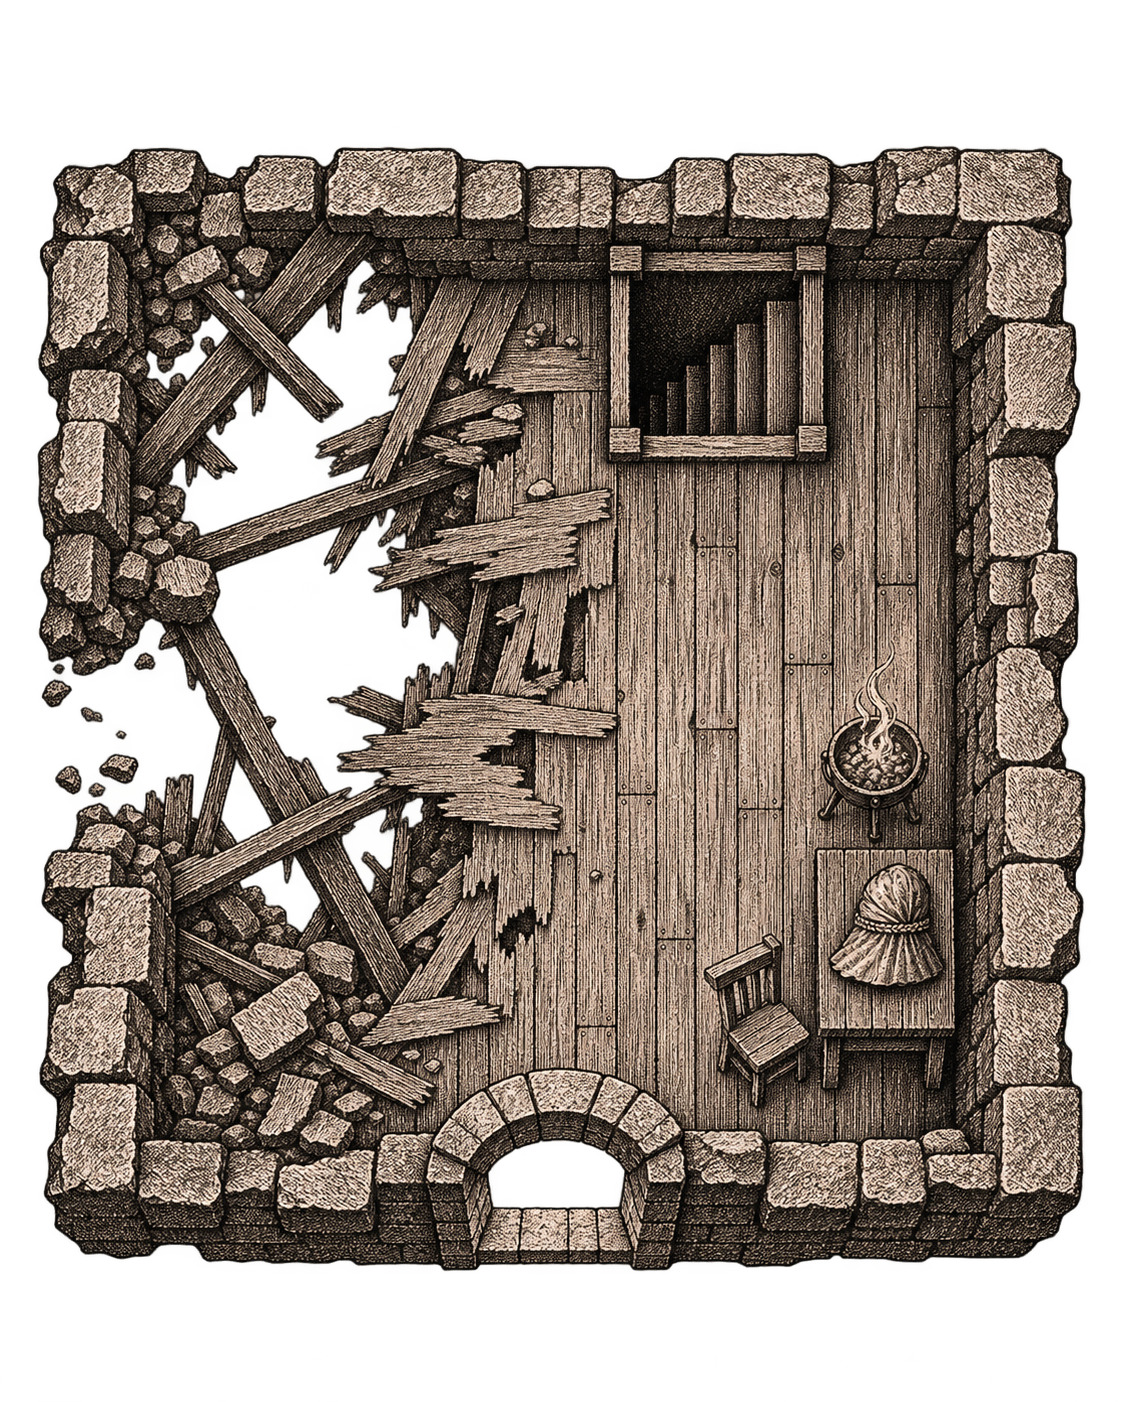
\includegraphics[width=.98\linewidth,height=70mm,keepaspectratio]{assets/hollow-hearth/map-upper.jpg}\par\vspace{2pt}
{\footnotesize\itshape\color{rpgbrown}La vecchia torre: piano superiore\par}
{\scriptsize Scala a nord; lato occidentale esposto; finestra a sud, campana e braciere sul lato est intatto.\par}
&
\centering\vspace{0pt}
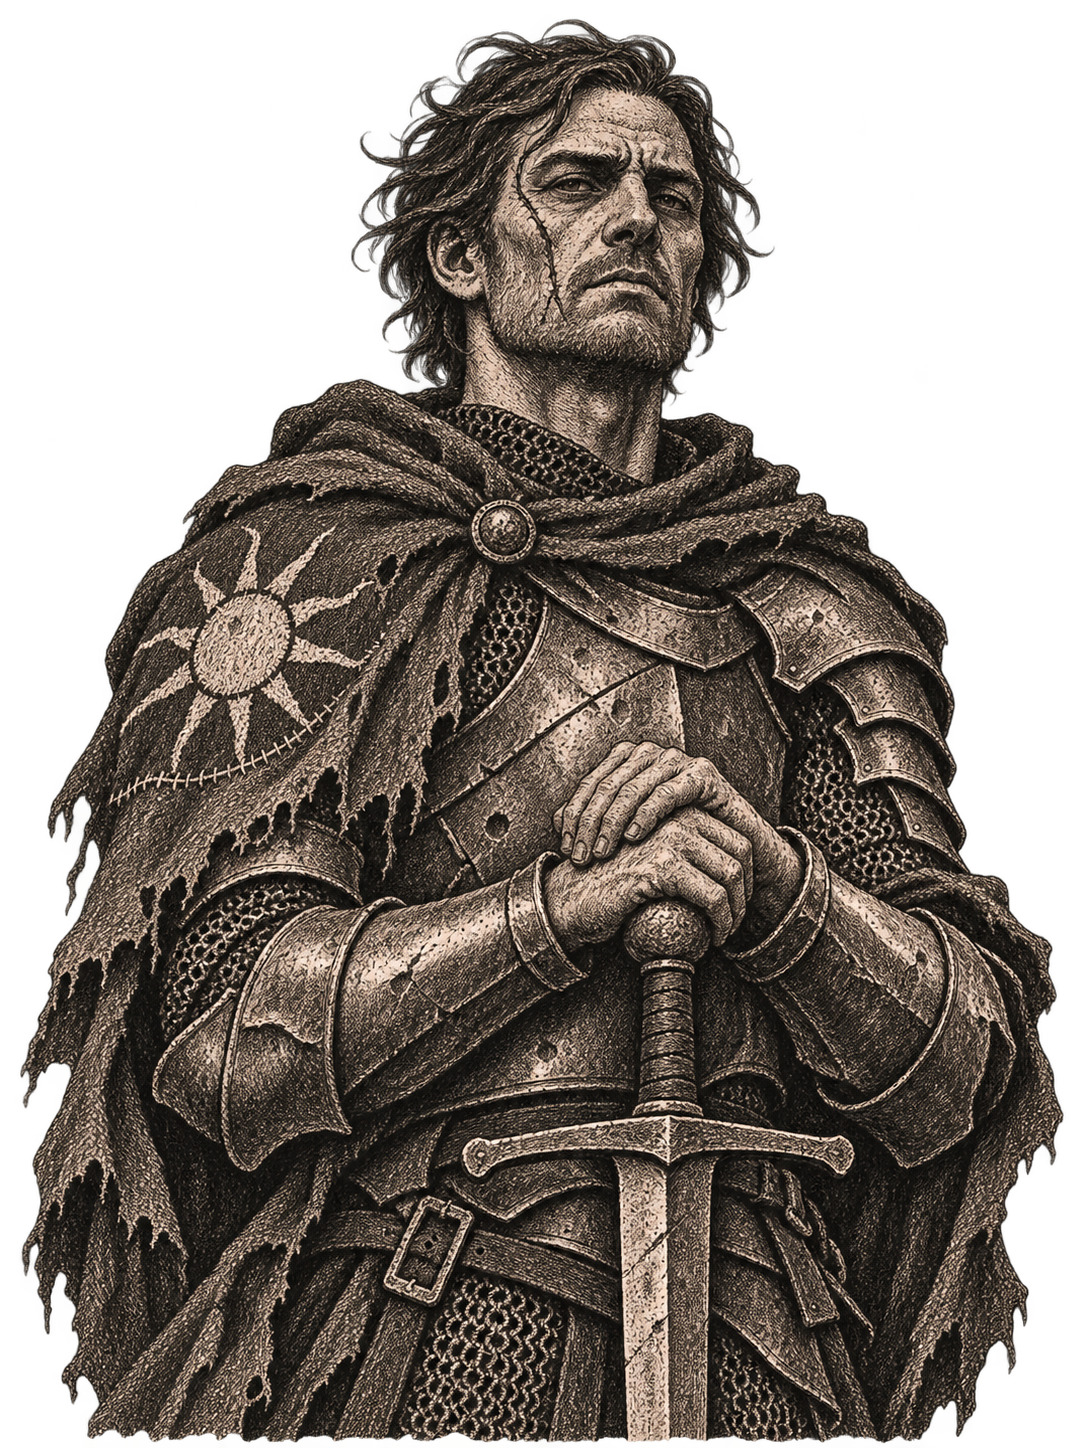
\includegraphics[width=.95\linewidth,height=68mm,keepaspectratio]{assets/hollow-hearth/corwin.jpg}\par\vspace{2pt}
{\footnotesize\itshape\color{rpgbrown}Ser Corwin Vask\par}
\end{tabular}
\par\medskip

Ser Corwin siede su una sedia di legno accanto alla \textbf{finestra a sud}, osservando il sentiero da cui salirà il compratore. La campana è accanto a lui su un tavolino, ancora avvolta nella tela cerata infangata. Un braciere di braci basse fornisce l'unica luce calda della stanza. La scala sbuca nella parete nord --- \textbf{alle sue spalle}.

La \textbf{metà occidentale del piano superiore è a cielo aperto}: lo stesso crollo che ha abbattuto il muro ovest del piano terra si è portato via la parte ovest del tetto e parte del pavimento a ovest. Travi allentate pendono di sbieco. Il pavimento esposto a ovest non è sicuro da attraversare senza cautela.

Questo crea un \textbf{quarto approccio}, che il testo precedente si limitava ad accennare:

\textbf{La scalata.} Un personaggio con \textbf{Acrobazia} può arrampicarsi sul cumulo di macerie del muro crollato al piano terra e proseguire lungo l'esterno della parete ovest spezzata, entrando dalla breccia nel tetto. Tira \textbf{Destrezza + Acrobazia, VR 4} per arrampicarsi senza problemi; senza Acrobazia, \textbf{VR 5}. Un fallimento significa cadere: 1 Ferita per l'altezza, più il rumore della caduta (Corwin lo sentirà). Con un successo, il personaggio si cala sul piano superiore \emph{alle spalle} di Corwin, cogliendolo di sorpresa. È un approccio per un solo personaggio: il Combattente in armatura pesante non può tentare la scalata, e un Mistico, con pochi PV, non può permettersi la caduta in caso di fallimento. \textbf{Un Avventuriero agile è il più adatto a questo approccio.}

\par\Needspace{12\baselineskip}\noindent\textbf{Elementi tattici del piano superiore:}

\begin{itemize}
\tightlist
\item
  \textbf{La finestra a sud.} Chiunque raggiunga la campana può scagliarla fuori: atterra pesantemente vicino al falò, di sotto, forse incrinata. Il compratore, che osserva dal sentiero, lo vedrà. Un Protagonista può anche usare la finestra per fuggire dalla stanza, calandosi a terra (Destrezza + Acrobazia, \textbf{VR 4} per atterrare senza danni; un fallimento costa 1 Ferita).
\item
  \textbf{La metà occidentale pericolante.} Chi combatte sulla metà crollata tira con una Condizione: \textbf{$-1$ gradino}. Un personaggio spinto oltre il bordo precipita di un piano (2 Ferite). Corwin, che conosce la stanza, combatterà solo sulla metà orientale, e cercherà volentieri di spingere i nemici sul terreno malfermo.
\item
  \textbf{Il braciere.} Se rovesciato, sparge braci sul pavimento di legno secco: il fuoco si propaga nell'arco di due scene d'azione e la stanza diventa inabitabile. Una mossa disperata, alla portata di chiunque, che può salvare il gruppo o distruggere la campana insieme a tutto il resto.
\item
  \textbf{L'armatura pesante di Ser Corwin.} La sua armatura pesante porta il VR per colpirlo a \textbf{4 con Forza} o \textbf{5 con Destrezza}. Non riduce il danno. Un braciere rovesciato, una spinta verso il bordo crollato o un Critico di un Protagonista che ha dichiarato Sforzo possono cambiare le sorti del confronto.
\end{itemize}

\subsubsection{Adattare lo scontro}\label{adattare-lo-scontro}

\begingroup\setlength{\arrayrulewidth}{.34pt}\arrayrulecolor{rpgline}\renewcommand{\arraystretch}{1.32}\rowcolors{2}{rpgshade}{white}\par\smallskip\noindent\begin{tabularx}{\linewidth}{|Y|Y|Y}\hline
\rpghead{Dimensione del gruppo} & \rpghead{Briganti} & \rpghead{Ser Corwin} \\ \hline
3 giocatori & 3 briganti (in gruppo) & Sì \\ \hline
4 giocatori & 4 briganti (2 fuori, 2 dentro) & Sì \\ \hline
\end{tabularx}\arrayrulecolor{black}\endgroup\par\smallskip

Se il gruppo sembra in seria difficoltà, fai fuggire un brigante al primo vero spargimento di sangue. Se invece passa oltre senza difficoltà, il compratore arriva in anticipo.

\subsubsection{Il colpo di scena · Il compratore}\label{il-colpo-di-scena-il-compratore}

Se il gruppo è ancora alla torre a \textbf{mezzanotte} --- che stia combattendo, trattando o abbia già vinto --- una figura ammantata esce dal bosco, da sola, senza volto sotto il cappuccio. \textbf{Il compratore è uno del Popolo Cavo sotto sembianze umane.} Vuole che la campana taccia per sempre, non che venga distrutta. Porta un sacchetto d'argento. Parla con le stesse voci non del tutto giuste che il gruppo ha udito a metà entrando nel bosco.

\par\smallskip\begin{rpgnote}[fontupper=\normalfont]\textbf{Il compratore (uno del Popolo Cavo sotto sembianze umane)} \emph{VR F3/D4 · Esperto · 4 Ferite · tocco (1S Prodigio; con un Critico, 2F + una Condizione che dura per il resto della scena) · nessuna armatura.} \emph{Comportamento: «Pronuncia le sillabe sbagliate. Gli alberi non rispondono. Sanguina linfa, non sangue».}\end{rpgnote}\par\smallskip
È un \textbf{momento di scelta}. Il gruppo può:

\begin{itemize}
\tightlist
\item
  \textbf{Rifiutare e combattere.} \emph{(Blocco statistiche qui sopra.)}
\item
  \textbf{Accettare l'argento.} Il gruppo se ne va ricco. Di Focolare Vuoto non si vedrà più anima viva. \emph{Se lo scelgono, lascia che sia un vero finale.}
\item
  \textbf{Mentire e tendere un'imboscata al compratore.} \textbf{Tiri di Sapienza contrapposti alla Sapienza (Esperto) del compratore}. Se il gruppo vince, tiene l'argento \emph{e} la campana, ma il bosco lo ha marchiato, e la prossima avventura comincia con quel marchio.
\end{itemize}

\subsubsection{Il culmine --- e l'ultimo tiro}\label{il-culmine-lultimo-tiro}

Qualunque strada venga scelta, il momento culminante dovrebbe lasciare almeno un Protagonista in stato \textbf{Malmesso} o \textbf{Grave}. Tieni d'occhio i PV al tavolo. Nell'istante in cui un giocatore scende a \textbf{1 PV} e ha ancora un tiro da fare per chiudere la scena, fermati. Guardalo da un capo all'altro del tavolo. Chiedi:

\begin{quote}
\emph{«Siamo all'ultimo tiro. Vuoi sanguinare pur di riuscirci?»}
\end{quote}

Accompagnalo nella dichiarazione dello \textbf{Sforzo} \emph{(manuale, p. 13)}. Lascialo tirare; la Ferita di Stanchezza arriva dopo il tiro. \textbf{È il momento da cui il gioco prende il nome.} Fallo sentire tale. Se il tiro riesce, il tavolo dovrebbe esultare. Se fallisce, il tavolo dovrebbe ammutolire.

\par\vspace{3pt}

\subsection{Risoluzione}\label{risoluzione}

Tre finali netti, con conseguenze che preparano la prossima avventura:

\textbf{La campana torna.} Hesta consegna la \textbf{Lama del Sale} e offre tutta l'ospitalità del villaggio. Se il gruppo le ha riportato il fiore, Vela lo annovera fra i suoi amici. La voce si sparge fino al paese successivo. \emph{La prossima avventura comincia con qualcuno che cerca il gruppo per nome.}

\textbf{La campana viene fatta tacere o venduta.} Il gruppo se ne va ricco e marchiato. Il Popolo Cavo ne prende nota. \emph{Una futura avventura comincia con sussurri notturni che conoscono i loro nomi.}

\textbf{La campana viene distrutta.} Per un Contraccolpo sfortunato o uno scontro disperato, il Popolo Cavo torna a Focolare Vuoto nella notte senza luna. \emph{La prossima avventura comincia con il gruppo che cerca di rimediare. Veyl Ashen, il Mistico delle origini, potrebbe non essere morto come raccontano le cronache.}

\subsubsection{Le tre domande}\label{le-tre-domande}

Concludi la sessione facendo rispondere il gruppo, insieme, alle tre domande dell'Avanzamento (manuale, p. 11). Il resoconto giusto è quello onesto, non quello generoso. Un giocatore alle prime armi che si è bloccato a ogni occasione non ha guadagnato punti avanzamento. Un giocatore alle prime armi che ha tentato, fallito e fatto i conti con le conseguenze ne ha guadagnati tre. Chiariscilo, con delicatezza, la prima volta.

\par\vspace{3pt}

\par\smallskip\section*{Promemoria del Narratore}\label{riferimento-rapido-del-narratore}\addcontentsline{toc}{section}{V. Promemoria del Narratore}
\begingroup\footnotesize\setlength{\arrayrulewidth}{.34pt}\arrayrulecolor{rpgline}\renewcommand{\arraystretch}{1.14}
\noindent\begin{minipage}[t]{.49\linewidth}
\begin{tabularx}{\linewidth}{|>{\hsize=.78\hsize}Y|>{\hsize=1.22\hsize}Y|}\hline
\rpghead{Situazione} & \rpghead{Regola / valore} \\ \hline
VR 3–6 & Semplice / Standard / Difficile / Estrema \\ \hline
Distanze & Addosso; Vicino; A portata; Lontano \\ \hline
Aiuto & Esperto o superiore: +1d6; inferiore: +1d6 e VR +1 \\ \hline
Sforzo & +1d6 prima del tiro; 1S dopo \\ \hline
Stato & $\le$ 2 PV: $-1$ gradino; $\le$ 1 PV: $-2$ gradini \\ \hline
\end{tabularx}
\end{minipage}\hfill
\begin{minipage}[t]{.49\linewidth}
\begin{tabularx}{\linewidth}{|>{\hsize=.78\hsize}Y|>{\hsize=1.22\hsize}Y|}\hline
\rpghead{Situazione} & \rpghead{Regola / valore} \\ \hline
Ponte & Destrezza VR 4; corda VR 3; caduta 2F \\ \hline
Seguire le tracce & Destrezza + Sopravvivenza, VR 4 \\ \hline
Furtività & Destrezza + Furtività, VR 4 \\ \hline
Scalata & Destrezza + Acrobazia, VR 4 (altrimenti 5) \\ \hline
Corwin & VR F4/D5; Esperto; 6F; spada 2F \\ \hline
\end{tabularx}
\end{minipage}
\arrayrulecolor{black}\endgroup


\HHAdventureBackCover
\end{document}
